\tikzset{circ/.style={circle, inner sep=0pt, minimum size=0.8cm, fill=blue!50, draw=black, text=white, align=center}}


\resizebox{\framewidth}{!}{%
\begin{tikzpicture}
 
    % MAIN RECTANGLE
    \node(main)[label={[label distance=1cm]above:\bfseries NEURAL NETWORK}] 
    {\tikz {\filldraw[thick,rounded corners=15pt,fill=orange!50] (-3,-2) rectangle (3,2);}};
        

    % INSIDE
    \node(first-circle)[circ, minimum size=1.4cm, thick] at (-0.5,1.1) {model \\ $w$};
    \node(second-circle)[circ, minimum size=1.4cm, thick] at (-0.5,-1.1) {model \\ $\hat{w}$};

    \draw[bend right,->, very thick, shorten <=2pt, shorten >=2pt]  (first-circle) to node [auto] 
    {\bfseries training $\mathbfcal{D}$ vs $\mathbfcal{R}$} (second-circle);

    \draw[thick] (-2.0,1.1) -- (first-circle);
    \node(point-1)[circ, minimum size=0.1cm, fill=black, label=left:{$\boldsymbol{x}$}] at (-2.0,1.1) {};

    \draw[thick] (first-circle) -- (1.0,1.1);
    \node(point-2)[circ, minimum size=0.1cm, fill=black, label=right:{$\boldsymbol{f(x;\,w)}$}] at (1.0,1.1) {};

    \draw[thick] (-2.0,-1.1) -- (second-circle);
    \node(point-3)[circ, minimum size=0.1cm, fill=black, label=left:{$\boldsymbol{x}$}] at (-2.0,-1.1) {};

    \draw[thick] (second-circle) -- (1.0,-1.1);
    \node(point-4)[circ, minimum size=0.1cm, fill=black, label=right:{$\boldsymbol{f(x;\,\hat{w})}$}] at (1.0,-1.1) {};


    % UPPER LEFT
    \node(ref)[above left = -1cm and 0cm of main, label={[label distance=-0.4cm]above:\bfseries reference sample $\mathbfcal{R}$}] 
    {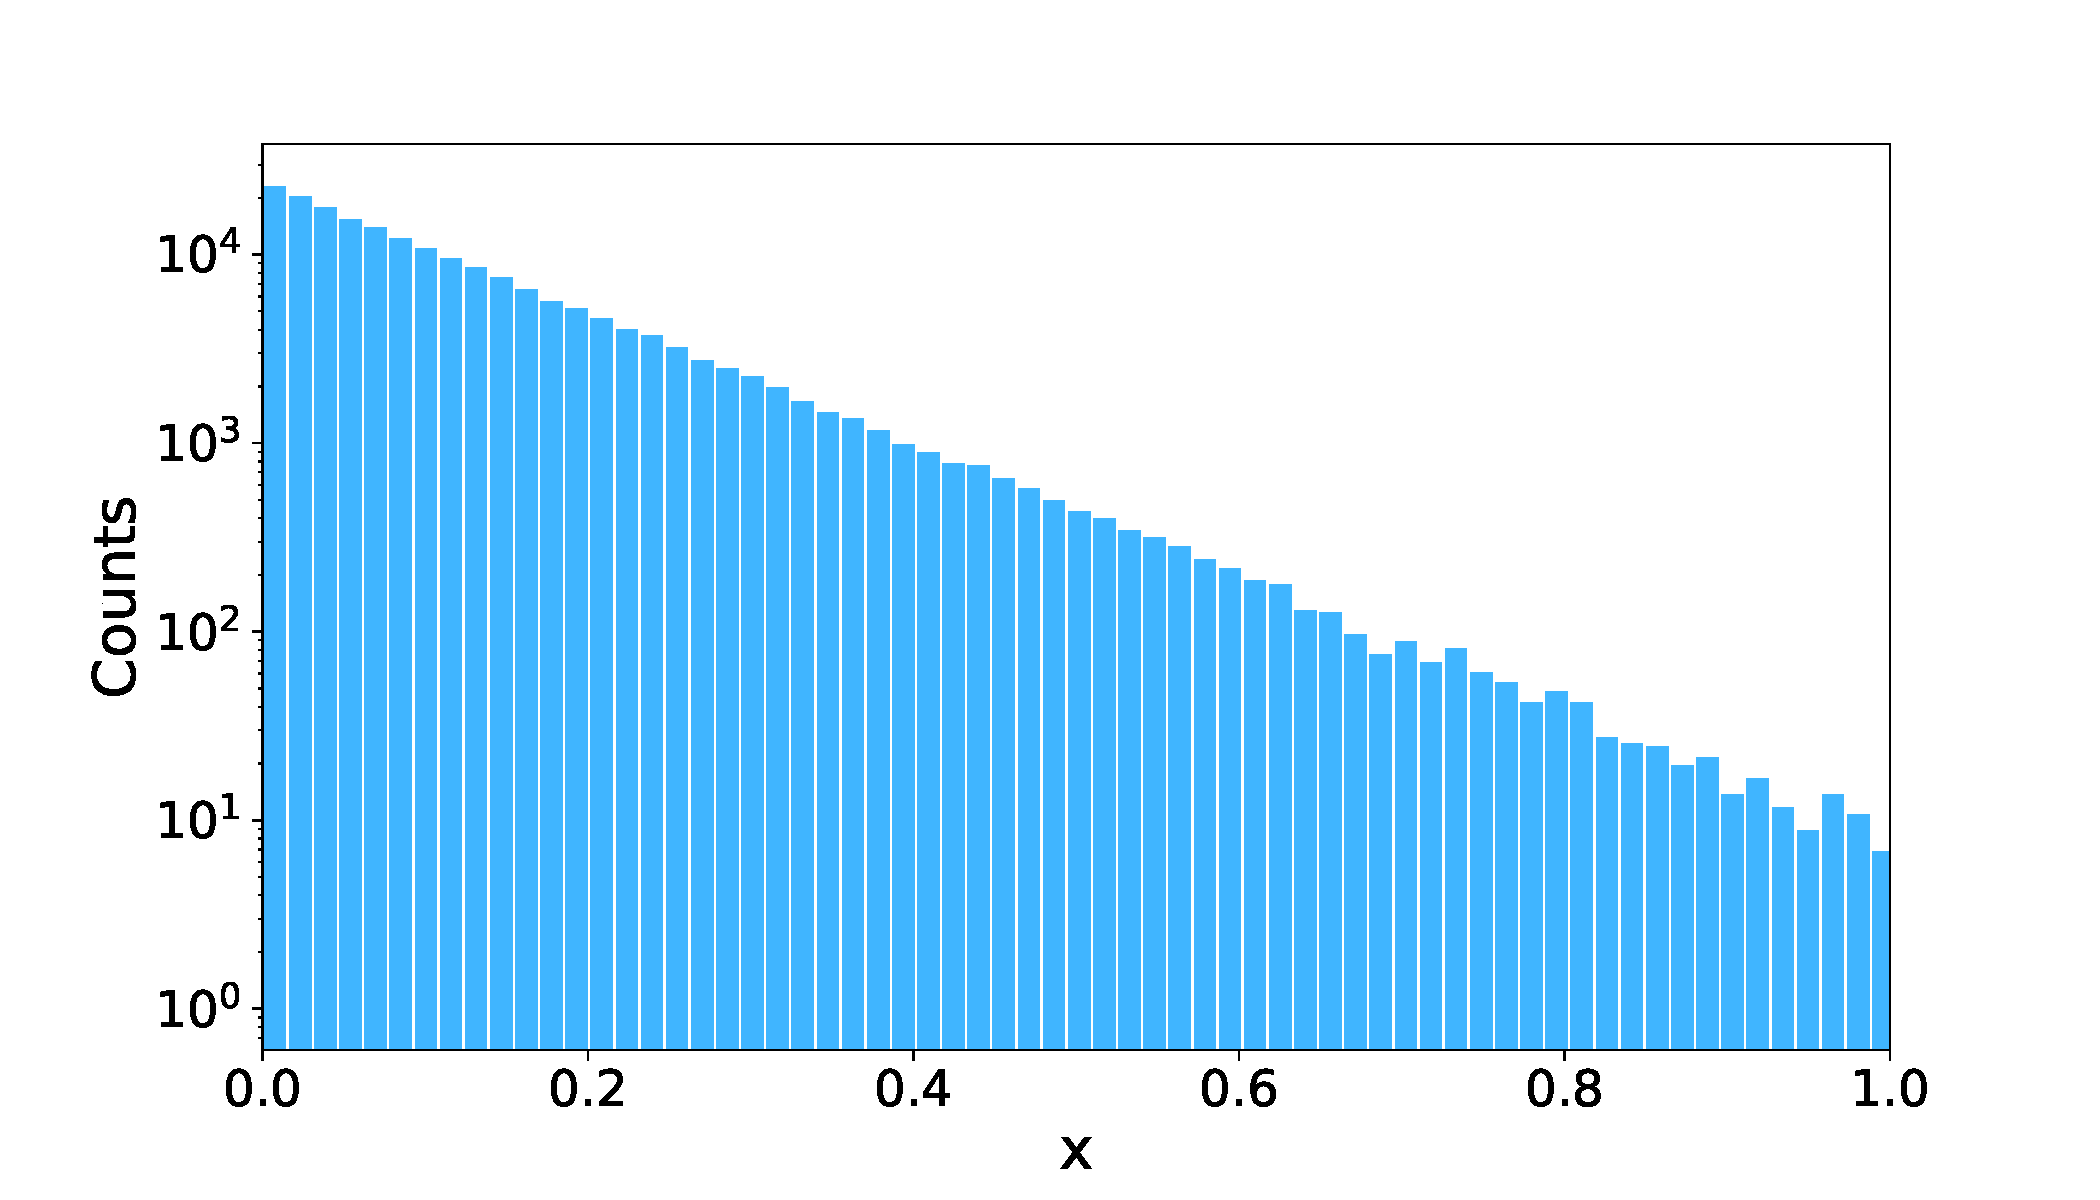
\includegraphics[width=.3\textwidth]{../PLOTS/DISTRIBUTIONS/ref.pdf}};
    \draw[bend left,->, very thick, shorten <=2pt, shorten >=2pt]  (ref) to node [auto] 
    {} (main);


    % LOWER LEFT
    \node(exp)[below left = -1cm and 0cm of main, label={[label distance=-0.4cm]above:\bfseries  data sample $\mathbfcal{D}$}]  
    {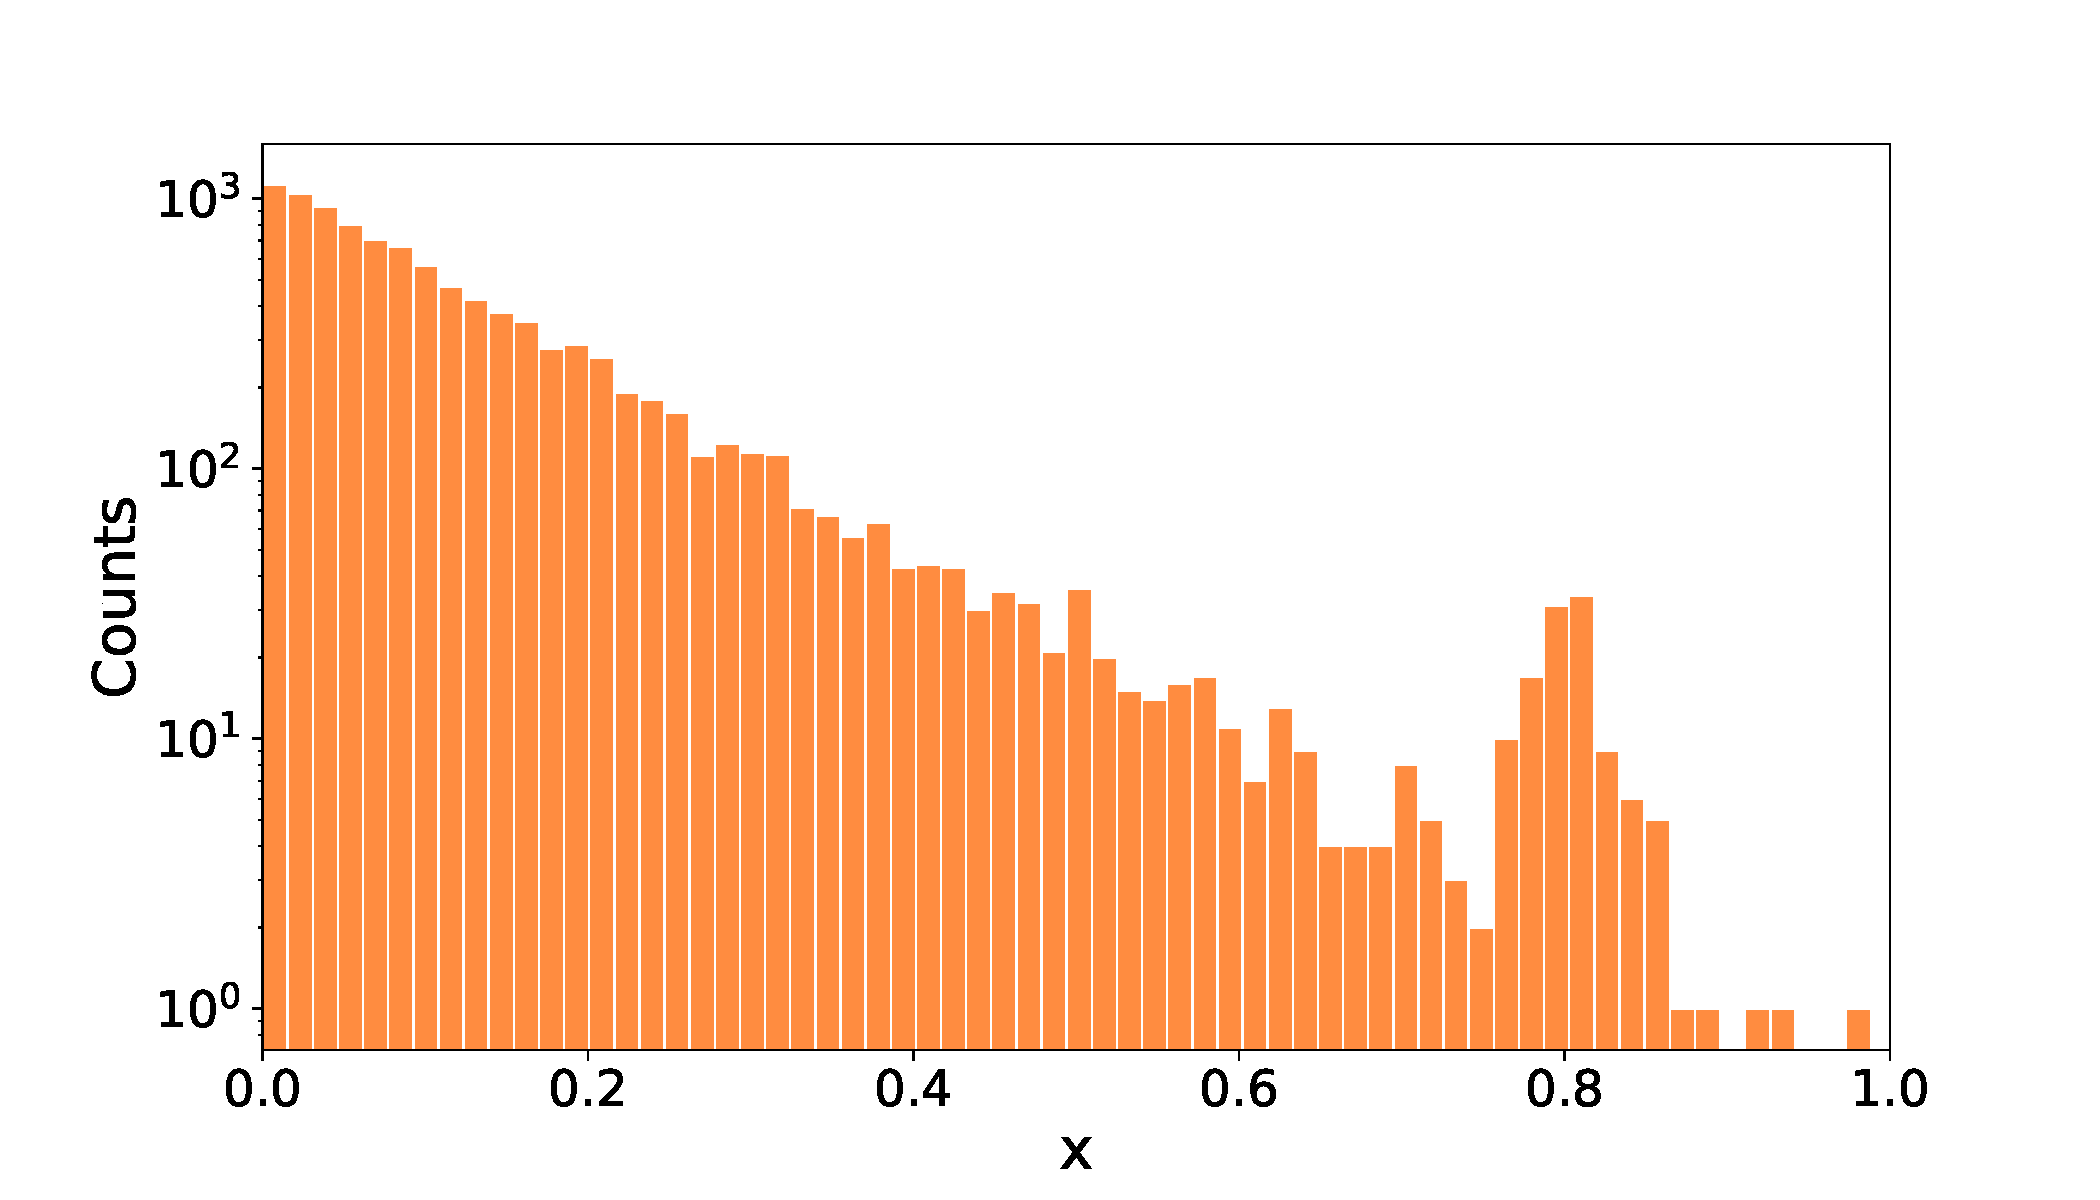
\includegraphics[width=.3\textwidth]{../PLOTS/DISTRIBUTIONS/exp.pdf}};
    \draw[bend right,->, very thick, shorten <=2pt, shorten >=2pt]  (exp) to node [auto] 
    {} (main);

    % UPPER RIGHT
    \node(log)[above right = -1cm and 0cm of main, label={[align=center, label distance=-0.4cm]above:\bfseries  log-ratio distribution \\ 
    $f(x;\,\hat{w})\approx \log\left[\frac{n(x\,|\,\mathbfcal{T})}{n(x\,|\,\mathbfcal{R})}\right]$}] 
    {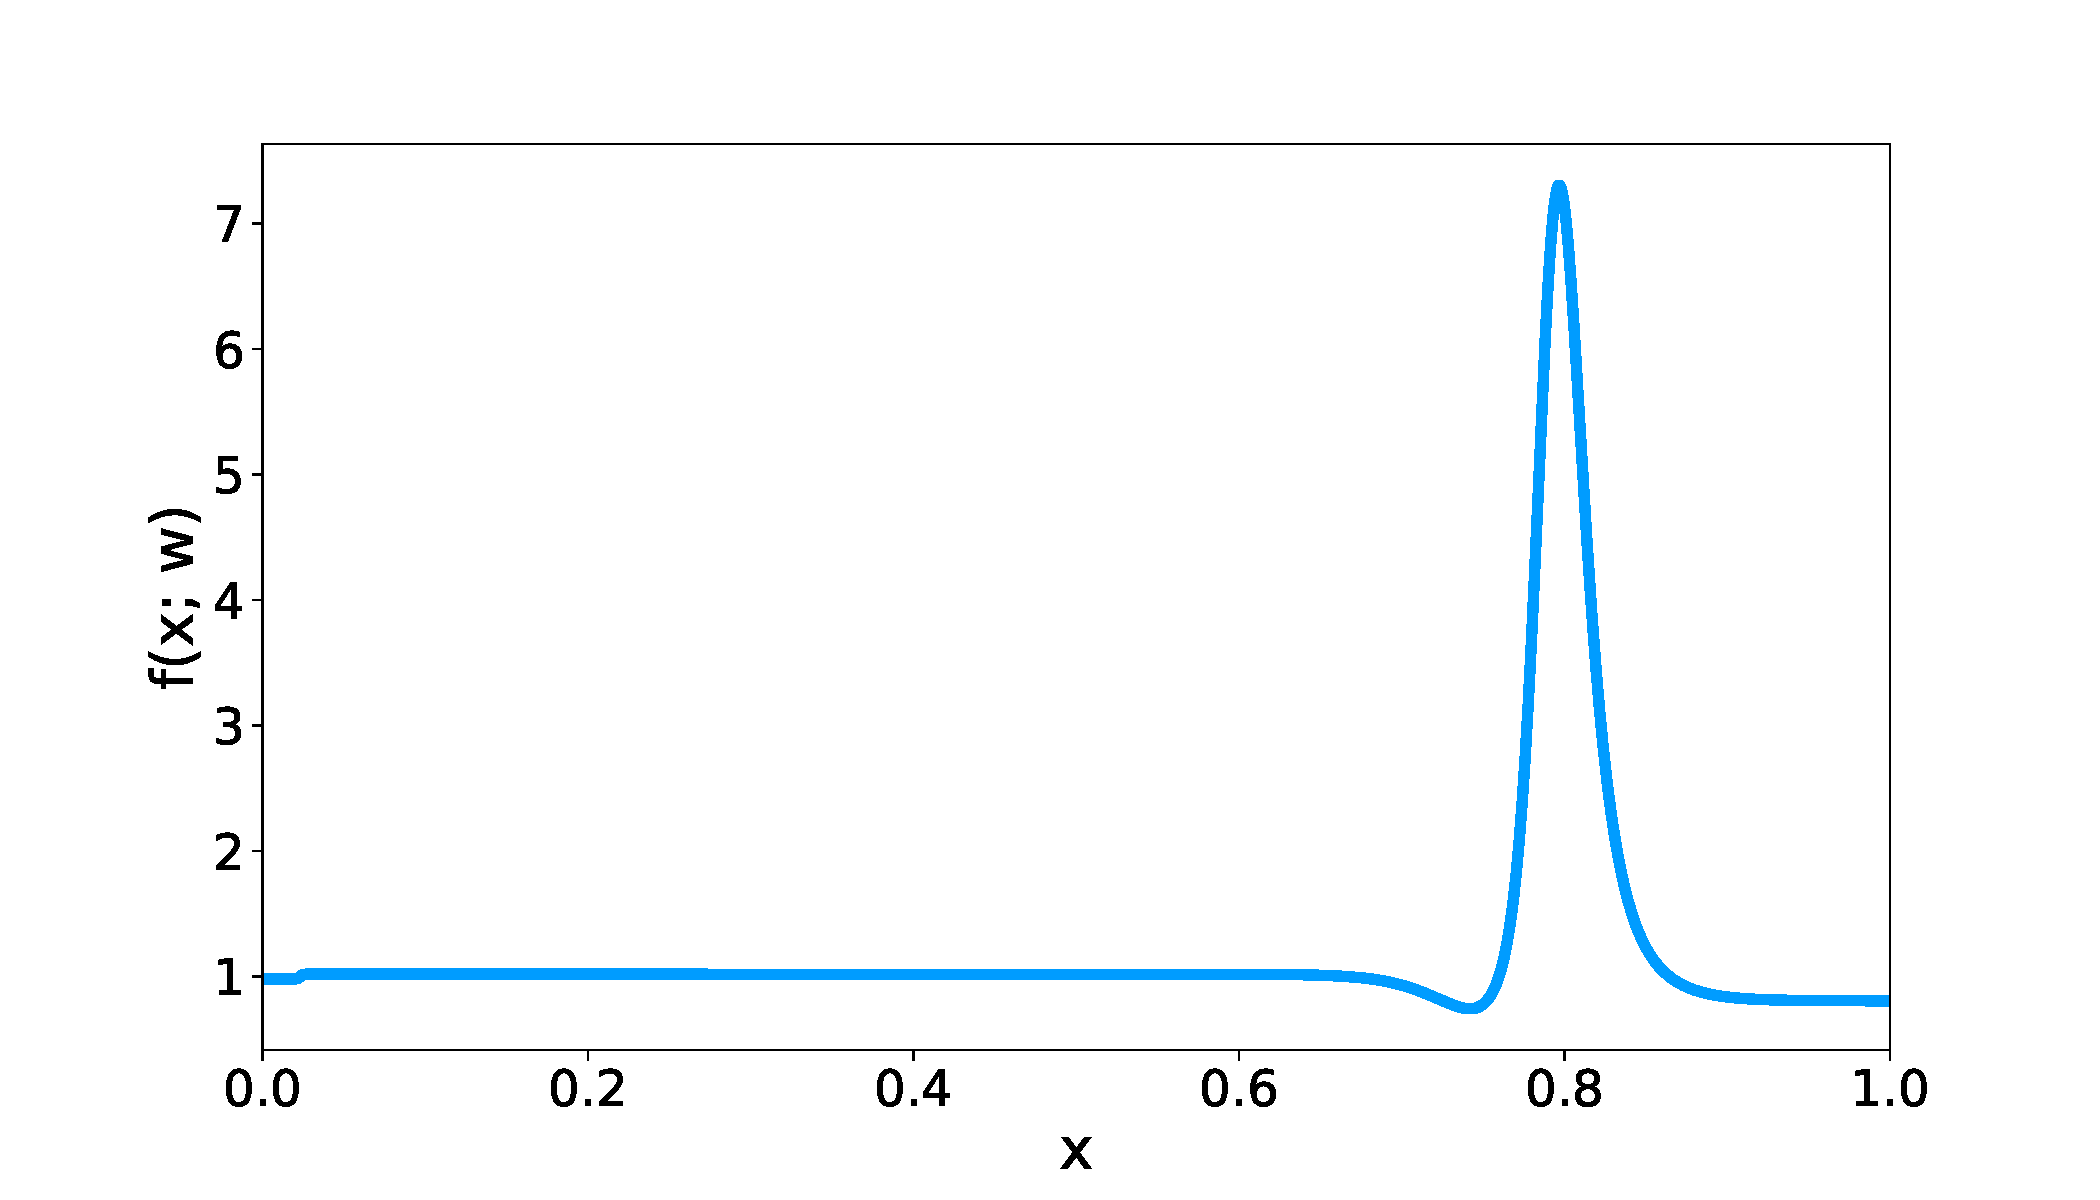
\includegraphics[width=.3\textwidth]{../PLOTS/DISTRIBUTIONS/log_ratio_47.pdf}};
    \draw[bend left,->, very thick, shorten <=2pt, shorten >=2pt]  (main) to node [auto] 
    {} (log);


    % LOWER RIGHT
    \node(t)[below right = -1cm and 0cm of main, label={[align=center, label distance=-0.4cm]above:\bfseries $\boldsymbol{t}$ distribution \\
    $t(\mathbfcal{D})=-2\,\min_w L[f]$}]  
    {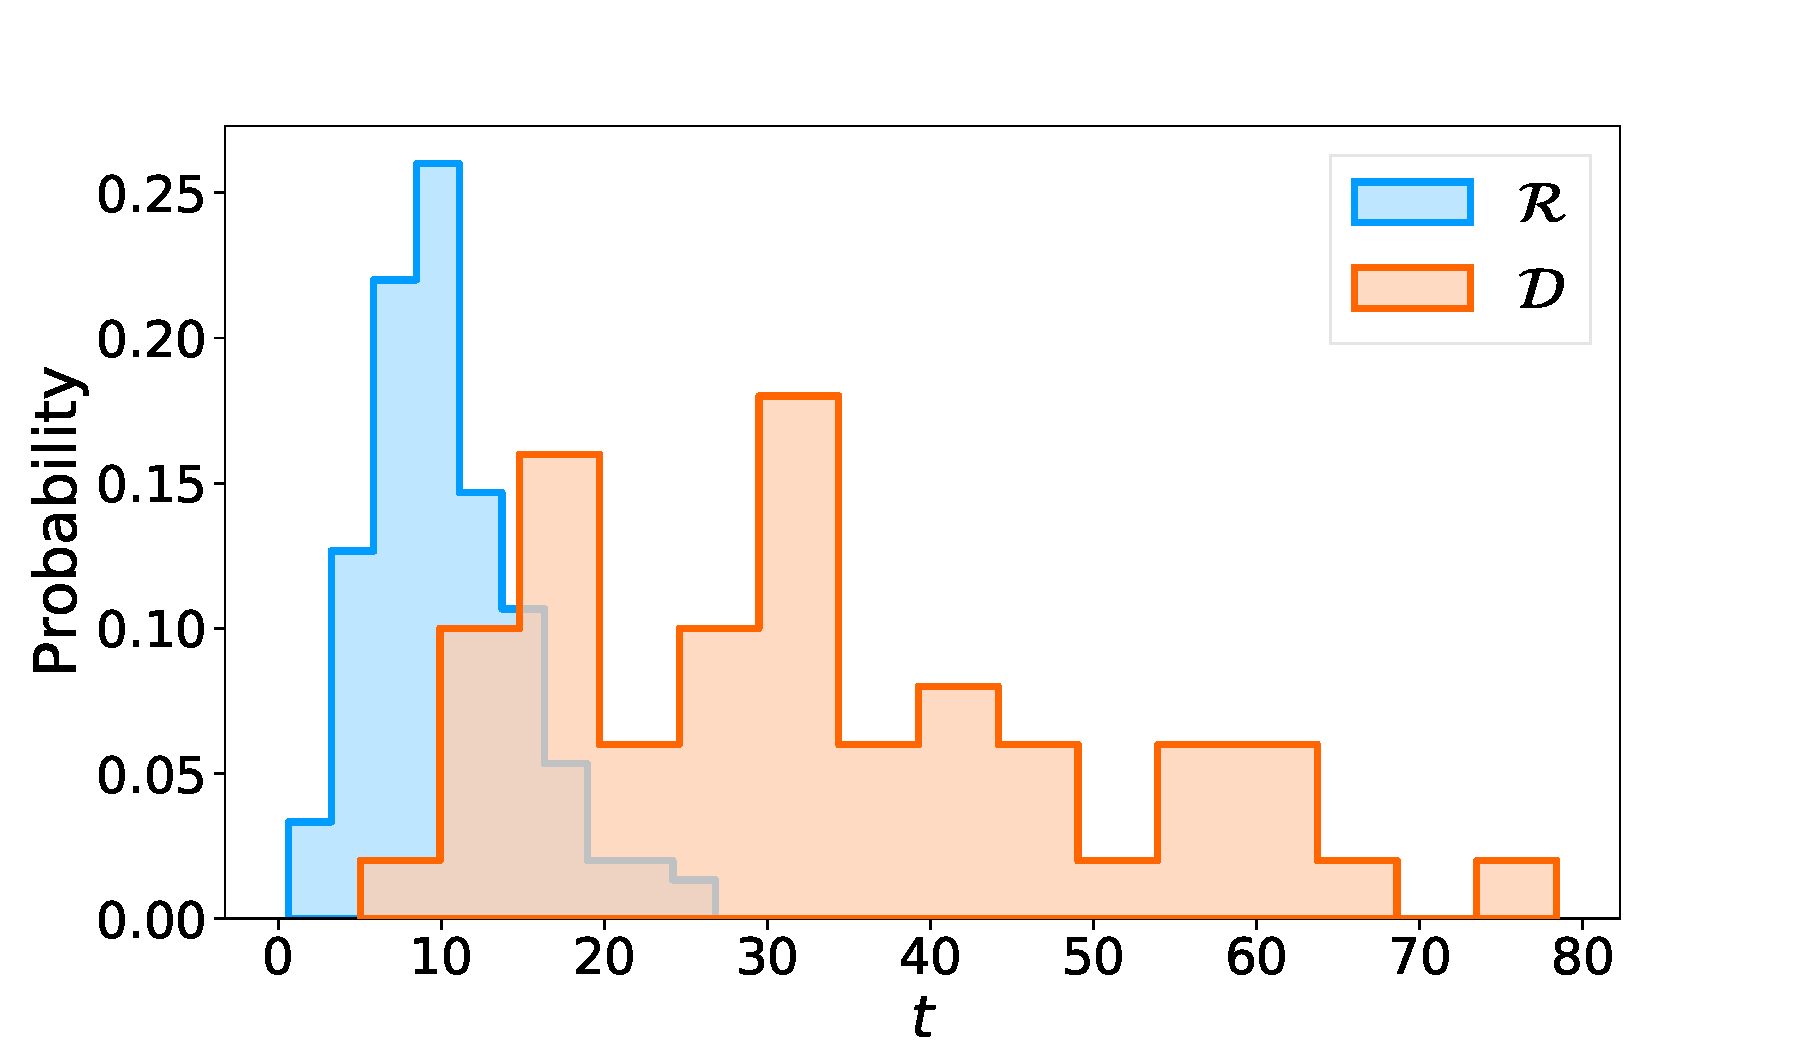
\includegraphics[width=.3\textwidth]{../PLOTS/DISTRIBUTIONS/summary_distribution.pdf}};
    \draw[bend right,->, very thick, shorten <=2pt, shorten >=2pt]  (main) to node [auto] 
    {} (t);

    % INPUT
    \node(in)[above = 1.5cm of ref]{\bfseries INPUT};

    % OUTPUT
    \node(out)[above = 1.5cm of log]{\bfseries OUTPUT};

\end{tikzpicture}}